\chapter{Kombinatorika}

\index{kombinatorika}

\key{Kombinatorika} proučava metode za prebrojavanje
kombinacija objekata.
Obično je cilj pronaći način da
kombinacije prebrojimo efikasno,
bez generiranja svake kombinacije zasebno.

Kao primjer, razmotrimo zadatak
prebrojavanja načina na koje
cijeli broj $n$ možemo prikazati kao sumu pozitivnih cijelih brojeva.
Na primjer, postoji 8 prikaza
broja $4$:
\begin{multicols}{2}
\begin{itemize}
\item $1+1+1+1$
\item $1+1+2$
\item $1+2+1$
\item $2+1+1$
\item $2+2$
\item $3+1$
\item $1+3$
\item $4$
\end{itemize}
\end{multicols}

Kombinatorni zadatak često se može riješiti
pomoću rekurzivne funkcije.
U ovom zadatku možemo definirati funkciju $f(n)$
koja daje broj prikaza broja $n$.
Na primjer, $f(4)=8$ prema gornjem primjeru.
Vrijednosti funkcije
mogu se rekurzivno izračunati na sljedeći način:
\begin{equation*}
    f(n) = \begin{cases}
               1               & n = 0\\
               f(0)+f(1)+\cdots+f(n-1) & n > 0\\
           \end{cases}
\end{equation*}
Bazni slučaj je $f(0)=1$,
jer prazna suma predstavlja broj 0.
Zatim, ako je $n>0$, razmatramo sve načine
odabira prvog broja u sumi.
Ako je prvi broj $k$,
postoji $f(n-k)$ prikaza
za preostali dio sume.
Stoga računamo sumu svih vrijednosti
oblika $f(n-k)$ gdje je $k<n$.

Prve vrijednosti funkcije su:
\[
\begin{array}{lcl}
f(0) & = & 1 \\
f(1) & = & 1 \\
f(2) & = & 2 \\
f(3) & = & 4 \\
f(4) & = & 8 \\
\end{array}
\]

Ponekad se rekurzivna formula može zamijeniti
formulom u zatvorenom obliku.
U ovom zadatku,
\[
f(n)=2^{n-1},
\]
što se temelji na činjenici da postoji $n-1$
mogućih pozicija za znakove + u sumi
i možemo odabrati bilo koji njihov podskup.

\section{Binomni koeficijenti}

\index{binomni koeficijent}

\key{Binomni koeficijent} ${n \choose k}$
jednak je broju načina na koje možemo odabrati podskup
od $k$ elemenata iz skupa od $n$ elemenata.
Na primjer, ${5 \choose 3}=10$,
jer skup $\{1,2,3,4,5\}$
ima 10 podskupova od 3 elementa:
\[ \{1,2,3\}, \{1,2,4\}, \{1,2,5\}, \{1,3,4\}, \{1,3,5\}, 
\{1,4,5\}, \{2,3,4\}, \{2,3,5\}, \{2,4,5\}, \{3,4,5\} \]

\subsubsection{Formula 1}

Binomni koeficijenti mogu se
rekurzivno izračunati na sljedeći način:

\[
{n \choose k}  =  {n-1 \choose k-1} + {n-1 \choose k}
\]

Ideja je fiksirati element $x$ u skupu.
Ako je $x$ uključen u podskup,
moramo odabrati $k-1$
elemenata od $n-1$ elemenata,
a ako $x$ nije uključen u podskup,
moramo odabrati $k$ elemenata od $n-1$ elemenata.

Bazni slučajevi rekurzije su
\[
{n \choose 0}  =  {n \choose n} = 1,
\]
jer uvijek postoji točno
jedan način da konstruiramo prazan podskup
i podskup koji sadrži sve elemente.

\subsubsection{Formula 2}

Drugi način izračuna binomnih koeficijenata je sljedeći:
\[
{n \choose k}  =  \frac{n!}{k!(n-k)!}.
\]

Postoji $n!$ permutacija od $n$ elemenata.
Prolazimo kroz sve permutacije i uvijek
uključujemo prvih $k$ elemenata permutacije
u podskup.
Budući da poredak elemenata u podskupu
i izvan podskupa nije bitan,
rezultat dijelimo s $k!$ i $(n-k)!$

\subsubsection{Svojstva}

Za binomne koeficijente vrijedi
\[
{n \choose k}  =  {n \choose n-k},
\]
jer zapravo dijelimo skup od $n$ elemenata na
dva podskupa: prvi sadrži $k$ elemenata,
a drugi sadrži $n-k$ elemenata.

Suma binomnih koeficijenata je
\[
{n \choose 0}+{n \choose 1}+{n \choose 2}+\ldots+{n \choose n}=2^n.
\]

Razlog za naziv ''binomni koeficijent''
vidi se kada binom $(a+b)$ podignemo na
$n$-tu potenciju:

\[ (a+b)^n =
{n \choose 0} a^n b^0 + 
{n \choose 1} a^{n-1} b^1 +
\ldots + 
{n \choose n-1} a^1 b^{n-1} +
{n \choose n} a^0 b^n. \]

\index{Pascalov trokut}

Binomni koeficijenti pojavljuju se i u
\key{Pascalovom trokutu}
gdje je svaka vrijednost jednaka sumi dviju
vrijednosti iznad nje:
\begin{center}
\begin{tikzpicture}{0.9}
\node at (0,0) {1};
\node at (-0.5,-0.5) {1};
\node at (0.5,-0.5) {1};
\node at (-1,-1) {1};
\node at (0,-1) {2};
\node at (1,-1) {1};
\node at (-1.5,-1.5) {1};
\node at (-0.5,-1.5) {3};
\node at (0.5,-1.5) {3};
\node at (1.5,-1.5) {1};
\node at (-2,-2) {1};
\node at (-1,-2) {4};
\node at (0,-2) {6};
\node at (1,-2) {4};
\node at (2,-2) {1};
\node at (-2,-2.5) {$\ldots$};
\node at (-1,-2.5) {$\ldots$};
\node at (0,-2.5) {$\ldots$};
\node at (1,-2.5) {$\ldots$};
\node at (2,-2.5) {$\ldots$};
\end{tikzpicture}
\end{center}

\subsubsection{Kutije i kuglice}

''Kutije i kuglice'' koristan je model
u kojem brojimo načine
raspoređivanja $k$ kuglica u $n$ kutija.
Razmotrimo tri scenarija:

\textit{Scenarij 1}: Svaka kutija može sadržavati
najviše jednu kuglicu.
Na primjer, kada je $n=5$ i $k=2$,
postoji 10 rješenja:

\begin{center}
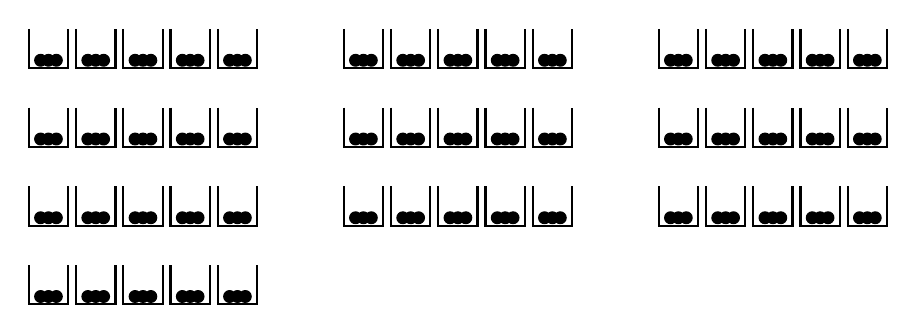
\begin{tikzpicture}[scale=0.5]
\newcommand\lax[3]{
\path[draw,thick,-] (#1-0.5,#2+0.5) -- (#1-0.5,#2-0.5) --
                    (#1+0.5,#2-0.5) -- (#1+0.5,#2+0.5);
\ifthenelse{\equal{#3}{1}}{\draw[fill=black] (#1,#2-0.3) circle (0.15);}{}
\ifthenelse{\equal{#3}{2}}{\draw[fill=black] (#1-0.2,#2-0.3) circle (0.15);}{}
\ifthenelse{\equal{#3}{2}}{\draw[fill=black] (#1+0.2,#2-0.3) circle (0.15);}{}
}
\newcommand\laa[7]{
    \lax{#1}{#2}{#3}
    \lax{#1+1.2}{#2}{#4}
    \lax{#1+2.4}{#2}{#5}
    \lax{#1+3.6}{#2}{#6}
    \lax{#1+4.8}{#2}{#7}
}

\laa{0}{0}{1}{1}{0}{0}{0}
\laa{0}{-2}{1}{0}{1}{0}{0}
\laa{0}{-4}{1}{0}{0}{1}{0}
\laa{0}{-6}{1}{0}{0}{0}{1}
\laa{8}{0}{0}{1}{1}{0}{0}
\laa{8}{-2}{0}{1}{0}{1}{0}
\laa{8}{-4}{0}{1}{0}{0}{1}
\laa{16}{0}{0}{0}{1}{1}{0}
\laa{16}{-2}{0}{0}{1}{0}{1}
\laa{16}{-4}{0}{0}{0}{1}{1}

\end{tikzpicture}
\end{center}

U ovom scenariju, odgovor je izravno
binomni koeficijent ${n \choose k}$.

\textit{Scenarij 2}: Kutija može sadržavati više kuglica.
Na primjer, kada je $n=5$ i $k=2$,
postoji 15 rješenja:

\begin{center}
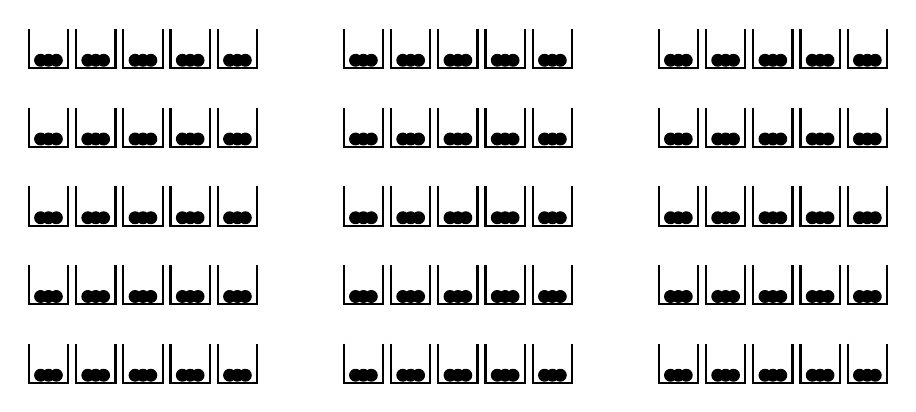
\begin{tikzpicture}[scale=0.5]
\newcommand\lax[3]{
\path[draw,thick,-] (#1-0.5,#2+0.5) -- (#1-0.5,#2-0.5) --
                    (#1+0.5,#2-0.5) -- (#1+0.5,#2+0.5);
\ifthenelse{\equal{#3}{1}}{\draw[fill=black] (#1,#2-0.3) circle (0.15);}{}
\ifthenelse{\equal{#3}{2}}{\draw[fill=black] (#1-0.2,#2-0.3) circle (0.15);}{}
\ifthenelse{\equal{#3}{2}}{\draw[fill=black] (#1+0.2,#2-0.3) circle (0.15);}{}
}
\newcommand\laa[7]{
    \lax{#1}{#2}{#3}
    \lax{#1+1.2}{#2}{#4}
    \lax{#1+2.4}{#2}{#5}
    \lax{#1+3.6}{#2}{#6}
    \lax{#1+4.8}{#2}{#7}
}

\laa{0}{0}{2}{0}{0}{0}{0}
\laa{0}{-2}{1}{1}{0}{0}{0}
\laa{0}{-4}{1}{0}{1}{0}{0}
\laa{0}{-6}{1}{0}{0}{1}{0}
\laa{0}{-8}{1}{0}{0}{0}{1}
\laa{8}{0}{0}{2}{0}{0}{0}
\laa{8}{-2}{0}{1}{1}{0}{0}
\laa{8}{-4}{0}{1}{0}{1}{0}
\laa{8}{-6}{0}{1}{0}{0}{1}
\laa{8}{-8}{0}{0}{2}{0}{0}
\laa{16}{0}{0}{0}{1}{1}{0}
\laa{16}{-2}{0}{0}{1}{0}{1}
\laa{16}{-4}{0}{0}{0}{2}{0}
\laa{16}{-6}{0}{0}{0}{1}{1}
\laa{16}{-8}{0}{0}{0}{0}{2}

\end{tikzpicture}
\end{center}

Postupak raspoređivanja kuglica u kutije
može se prikazati kao znakovni niz
koji se sastoji od simbola
''o'' i ''$\rightarrow$''.
Na početku pretpostavimo da stojimo kod krajnje lijeve kutije.
Simbol ''o'' znači da stavljamo kuglicu
u trenutnu kutiju, a simbol
''$\rightarrow$'' znači da se pomičemo
na sljedeću kutiju udesno.

Koristeći ovu notaciju, svako rješenje je znakovni niz
koji sadrži $k$ puta simbol ''o'' i
$n-1$ puta simbol ''$\rightarrow$''.
Na primjer, rješenje gore desno
na gornjoj slici odgovara znakovnom nizu
''$\rightarrow$ $\rightarrow$ o $\rightarrow$ o $\rightarrow$''.
Stoga je broj rješenja
${k+n-1 \choose k}$.

\textit{Scenarij 3}: Svaka kutija može sadržavati najviše jednu kuglicu,
i dodatno, nikoje dvije susjedne kutije ne smiju obje sadržavati kuglicu.
Na primjer, kada je $n=5$ i $k=2$,
postoji 6 rješenja:


\begin{center}
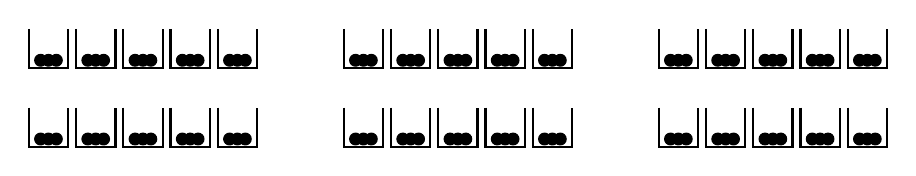
\begin{tikzpicture}[scale=0.5]
\newcommand\lax[3]{
\path[draw,thick,-] (#1-0.5,#2+0.5) -- (#1-0.5,#2-0.5) --
                    (#1+0.5,#2-0.5) -- (#1+0.5,#2+0.5);
\ifthenelse{\equal{#3}{1}}{\draw[fill=black] (#1,#2-0.3) circle (0.15);}{}
\ifthenelse{\equal{#3}{2}}{\draw[fill=black] (#1-0.2,#2-0.3) circle (0.15);}{}
\ifthenelse{\equal{#3}{2}}{\draw[fill=black] (#1+0.2,#2-0.3) circle (0.15);}{}
}
\newcommand\laa[7]{
    \lax{#1}{#2}{#3}
    \lax{#1+1.2}{#2}{#4}
    \lax{#1+2.4}{#2}{#5}
    \lax{#1+3.6}{#2}{#6}
    \lax{#1+4.8}{#2}{#7}
}

\laa{0}{0}{1}{0}{1}{0}{0}
\laa{0}{-2}{1}{0}{0}{1}{0}
\laa{8}{0}{1}{0}{0}{0}{1}
\laa{8}{-2}{0}{1}{0}{1}{0}
\laa{16}{0}{0}{1}{0}{0}{1}
\laa{16}{-2}{0}{0}{1}{0}{1}
\end{tikzpicture}
\end{center}

U ovom scenariju možemo pretpostaviti da je
$k$ kuglica na početku raspoređeno u kutije
i da se između svake dvije susjedne kutije
nalazi prazna kutija.
Preostali zadatak je odabrati
pozicije za preostale prazne kutije.
Takvih kutija ima $n-2k+1$, a
pozicija za njih ima $k+1$.
Stoga, koristeći formulu iz scenarija 2,
broj rješenja je
${n-k+1 \choose n-2k+1}$.

\subsubsection{Multinomni koeficijenti}

\index{multinomni koeficijent}

\key{Multinomni koeficijent}
\[ {n \choose k_1,k_2,\ldots,k_m} = \frac{n!}{k_1! k_2! \cdots k_m!}, \]
jednak je broju načina na koje
možemo podijeliti $n$ elemenata u podskupove
veličina $k_1,k_2,\ldots,k_m$,
gdje je $k_1+k_2+\cdots+k_m=n$.
Multinomni koeficijenti mogu se promatrati kao
generalizacija binomnih koeficijenata;
ako je $m=2$, gornja formula
odgovara formuli za binomni koeficijent.

\section{Catalanovi brojevi}

\index{Catalanov broj}

\key{Catalanov broj}
%\footnote{E. C. Catalan (1814--1894) was a Belgian mathematician.}
$C_n$ jednak je
broju valjanih
zagradnih izraza koji se sastoje od
$n$ lijevih zagrada i $n$ desnih zagrada.

Na primjer, $C_3=5$, jer
možemo konstruirati sljedeće zagradne
izraze koristeći tri
lijeve i desne zagrade:

\begin{itemize}[noitemsep]
\item \texttt{()()()}
\item \texttt{(())()}
\item \texttt{()(())}
\item \texttt{((()))}
\item \texttt{(()())}
\end{itemize}

\subsubsection{Zagradni izrazi}

\index{zagradni izraz}

Što je točno \emph{valjani zagradni izraz}?
Sljedeća pravila precizno definiraju sve
valjane zagradne izraze:

\begin{itemize}
\item Prazan zagradni izraz je valjan.
\item Ako je izraz $A$ valjan,
tada je i izraz
\texttt{(}$A$\texttt{)} valjan.
\item Ako su izrazi $A$ i $B$ valjani,
tada je i izraz $AB$ valjan.
\end{itemize}

Drugi način karakterizacije valjanih
zagradnih izraza jest da,
odaberemo li bilo koji prefiks takvog izraza,
on mora sadržavati barem onoliko lijevih
zagrada koliko i desnih zagrada.
Osim toga, cijeli izraz mora
sadržavati jednak broj lijevih i desnih
zagrada.

\subsubsection{Formula 1}

Catalanovi brojevi mogu se izračunati pomoću formule
\[ C_n = \sum_{i=0}^{n-1} C_{i} C_{n-i-1}.\]

Suma prolazi kroz načine podjele
izraza na dva dijela
tako da su oba dijela valjani
izrazi i da je prvi dio što kraći,
ali ne prazan.
Za bilo koji $i$, prvi dio sadrži $i+1$ parova
zagrada, a broj izraza
umnožak je sljedećih vrijednosti:

\begin{itemize}
\item $C_{i}$: broj načina konstruiranja izraza
pomoću zagrada prvog dijela,
ne računajući vanjske zagrade
\item $C_{n-i-1}$: broj načina konstruiranja
izraza pomoću zagrada drugog dijela
\end{itemize}

Bazni slučaj je $C_0=1$,
jer prazan zagradni izraz
možemo konstruirati pomoću nula parova zagrada.

\subsubsection{Formula 2}

Catalanovi brojevi mogu se izračunati
i pomoću binomnih koeficijenata:
\[ C_n = \frac{1}{n+1} {2n \choose n}\]
Formula se može objasniti na sljedeći način:

Postoji ukupno ${2n \choose n}$ načina
za konstruiranje (ne nužno valjanog)
zagradnog izraza koji sadrži $n$ lijevih
zagrada i $n$ desnih zagrada.
Izračunajmo broj takvih
izraza koji \emph{nisu} valjani.

Ako zagradni izraz nije valjan,
mora sadržavati prefiks u kojem
broj desnih zagrada premašuje
broj lijevih zagrada.
Ideja je obrnuti svaku zagradu
koja pripada takvom prefiksu.
Na primjer, izraz
\texttt{())()(} sadrži prefiks \texttt{())},
i nakon obrtanja prefiksa,
izraz postaje \texttt{)((()(}.

Rezultirajući izraz sastoji se od $n+1$
lijevih zagrada i $n-1$ desnih zagrada.
Broj takvih izraza je ${2n \choose n+1}$,
što je jednako broju nevaljanih
zagradnih izraza.
Stoga se broj valjanih zagradnih
izraza može izračunati pomoću formule
\[{2n \choose n}-{2n \choose n+1} = {2n \choose n} - \frac{n}{n+1} {2n \choose n} = \frac{1}{n+1} {2n \choose n}.\]

\subsubsection{Prebrojavanje stabala}

Catalanovi brojevi povezani su i sa stablima:

\begin{itemize}
\item postoji $C_n$ binarnih stabala s $n$ čvorova
\item postoji $C_{n-1}$ korijenskih stabala s $n$ čvorova
\end{itemize}
\noindent
Na primjer, za $C_3=5$, binarna stabla su

\begin{center}
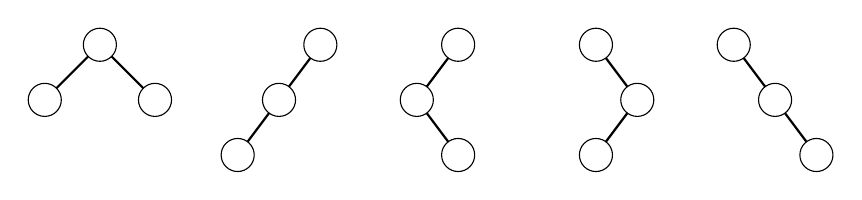
\begin{tikzpicture}[scale=0.7]
\path[draw,thick,-] (0,0) -- (-1,-1);
\path[draw,thick,-] (0,0) -- (1,-1);
\draw[fill=white] (0,0) circle (0.3);
\draw[fill=white] (-1,-1) circle (0.3);
\draw[fill=white] (1,-1) circle (0.3);

\path[draw,thick,-] (4,0) -- (4-0.75,-1) -- (4-1.5,-2);
\draw[fill=white] (4,0) circle (0.3);
\draw[fill=white] (4-0.75,-1) circle (0.3);
\draw[fill=white] (4-1.5,-2) circle (0.3);

\path[draw,thick,-] (6.5,0) -- (6.5-0.75,-1) -- (6.5-0,-2);
\draw[fill=white] (6.5,0) circle (0.3);
\draw[fill=white] (6.5-0.75,-1) circle (0.3);
\draw[fill=white] (6.5-0,-2) circle (0.3);

\path[draw,thick,-] (9,0) -- (9+0.75,-1) -- (9-0,-2);
\draw[fill=white] (9,0) circle (0.3);
\draw[fill=white] (9+0.75,-1) circle (0.3);
\draw[fill=white] (9-0,-2) circle (0.3);

\path[draw,thick,-] (11.5,0) -- (11.5+0.75,-1) -- (11.5+1.5,-2);
\draw[fill=white] (11.5,0) circle (0.3);
\draw[fill=white] (11.5+0.75,-1) circle (0.3);
\draw[fill=white] (11.5+1.5,-2) circle (0.3);
\end{tikzpicture}
\end{center}
a korijenska stabla su
\begin{center}
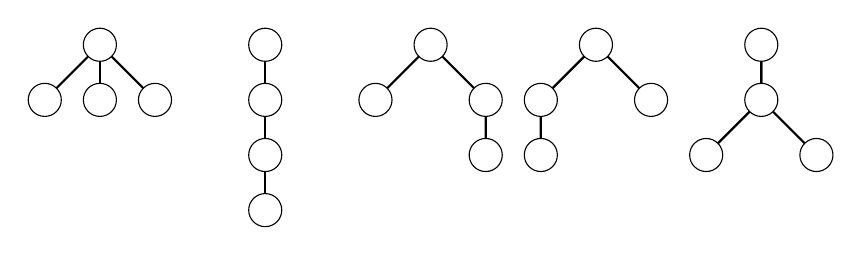
\begin{tikzpicture}[scale=0.7]
\path[draw,thick,-] (0,0) -- (-1,-1);
\path[draw,thick,-] (0,0) -- (0,-1);
\path[draw,thick,-] (0,0) -- (1,-1);
\draw[fill=white] (0,0) circle (0.3);
\draw[fill=white] (-1,-1) circle (0.3);
\draw[fill=white] (0,-1) circle (0.3);
\draw[fill=white] (1,-1) circle (0.3);

\path[draw,thick,-] (3,0) -- (3,-1) -- (3,-2) -- (3,-3);
\draw[fill=white] (3,0) circle (0.3);
\draw[fill=white] (3,-1) circle (0.3);
\draw[fill=white] (3,-2) circle (0.3);
\draw[fill=white] (3,-3) circle (0.3);

\path[draw,thick,-] (6+0,0) -- (6-1,-1);
\path[draw,thick,-] (6+0,0) -- (6+1,-1) -- (6+1,-2);
\draw[fill=white] (6+0,0) circle (0.3);
\draw[fill=white] (6-1,-1) circle (0.3);
\draw[fill=white] (6+1,-1) circle (0.3);
\draw[fill=white] (6+1,-2) circle (0.3);

\path[draw,thick,-] (9+0,0) -- (9+1,-1);
\path[draw,thick,-] (9+0,0) -- (9-1,-1) -- (9-1,-2);
\draw[fill=white] (9+0,0) circle (0.3);
\draw[fill=white] (9+1,-1) circle (0.3);
\draw[fill=white] (9-1,-1) circle (0.3);
\draw[fill=white] (9-1,-2) circle (0.3);

\path[draw,thick,-] (12+0,0) -- (12+0,-1) -- (12-1,-2);
\path[draw,thick,-] (12+0,0) -- (12+0,-1) -- (12+1,-2);
\draw[fill=white] (12+0,0) circle (0.3);
\draw[fill=white] (12+0,-1) circle (0.3);
\draw[fill=white] (12-1,-2) circle (0.3);
\draw[fill=white] (12+1,-2) circle (0.3);

\end{tikzpicture}
\end{center}

\section{Uključivanje-isključivanje}

\index{uključivanje-isključivanje}

\key{Uključivanje-isključivanje} je tehnika
koja se može koristiti za računanje veličine
unije skupova kada su poznate veličine
presjeka, i obrnuto.
Jednostavan primjer ove tehnike je formula
\[ |A \cup B| = |A| + |B| - |A \cap B|,\]
gdje su $A$ i $B$ skupovi, a $|X|$
označava veličinu skupa $X$.
Formula se može ilustrirati na sljedeći način:

\begin{center}
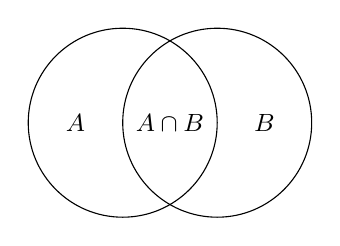
\begin{tikzpicture}[scale=0.8]

\draw (0,0) circle (1.5);
\draw (1.5,0) circle (1.5);

\node at (-0.75,0) {\small $A$};
\node at (2.25,0) {\small $B$};
\node at (0.75,0) {\small $A \cap B$};

\end{tikzpicture}
\end{center}

Naš cilj je izračunati
veličinu unije $A \cup B$
koja odgovara površini područja
koje pripada barem jednoj kružnici.
Slika pokazuje da površinu
$A \cup B$ možemo izračunati tako da prvo zbrojimo
površine $A$ i $B$, a zatim oduzmemo
površinu $A \cap B$.

Ista ideja može se primijeniti kada je broj
skupova veći.
Kada postoje tri skupa, formula uključivanja-isključivanja je
\[ |A \cup B \cup C| = |A| + |B| + |C| - |A \cap B|  - |A \cap C|  - |B \cap C| + |A \cap B \cap C| \]
a odgovarajuća slika je

\begin{center}
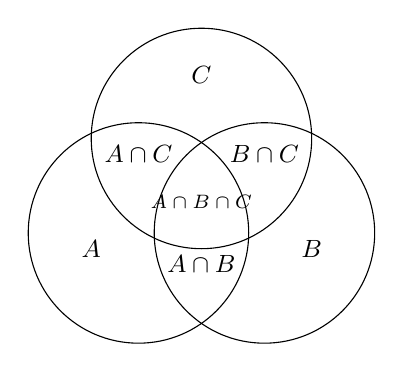
\begin{tikzpicture}[scale=0.8]

\draw (0,0) circle (1.75);
\draw (2,0) circle (1.75);
\draw (1,1.5) circle (1.75);

\node at (-0.75,-0.25) {\small $A$};
\node at (2.75,-0.25) {\small $B$};
\node at (1,2.5) {\small $C$};
\node at (1,-0.5) {\small $A \cap B$};
\node at (0,1.25) {\small $A \cap C$};
\node at (2,1.25) {\small $B \cap C$};
\node at (1,0.5) {\scriptsize $A \cap B \cap C$};

\end{tikzpicture}
\end{center}

U općem slučaju, veličina
unije $X_1 \cup X_2 \cup \cdots \cup X_n$
može se izračunati prolaskom kroz sve moguće
presjeke koji sadrže neke od skupova $X_1,X_2,\ldots,X_n$.
Ako presjek sadrži neparan broj skupova,
njegova veličina dodaje se odgovoru,
a inače se njegova veličina oduzima od odgovora.

Primijetimo da postoje slične formule
za računanje
veličine presjeka iz veličina
unija. Na primjer,
\[ |A \cap B| = |A| + |B| - |A \cup B|\]
i
\[ |A \cap B \cap C| = |A| + |B| + |C| - |A \cup B|  - |A \cup C|  - |B \cup C| + |A \cup B \cup C| .\]

\subsubsection{Deranžmani}

\index{deranžman}

Kao primjer, prebrojimo \key{deranžmane}
elemenata $\{1,2,\ldots,n\}$, tj. permutacije
u kojima nijedan element ne ostaje na svom izvornom mjestu.
Na primjer, kada je $n=3$, postoje
dva deranžmana: $(2,3,1)$ i $(3,1,2)$.

Jedan pristup rješavanju ovog zadatka je korištenje
uključivanja-isključivanja.
Neka je $X_k$ skup permutacija
koje sadrže element $k$ na poziciji $k$.
Na primjer, kada je $n=3$, skupovi su sljedeći:
\[
\begin{array}{lcl}
X_1 & = & \{(1,2,3),(1,3,2)\} \\
X_2 & = & \{(1,2,3),(3,2,1)\} \\
X_3 & = & \{(1,2,3),(2,1,3)\} \\
\end{array}
\]
Koristeći ove skupove, broj deranžmana jednak je
\[ n! - |X_1 \cup X_2 \cup \cdots \cup X_n|, \]
pa je dovoljno izračunati veličinu unije.
Koristeći uključivanje-isključivanje, to se svodi na
računanje veličina presjeka, što se može
učiniti efikasno.
Na primjer, kada je $n=3$, veličina
$|X_1 \cup X_2 \cup X_3|$ je
\[
\begin{array}{lcl}
 & & |X_1| + |X_2| + |X_3| - |X_1 \cap X_2|  - |X_1 \cap X_3|  - |X_2 \cap X_3| + |X_1 \cap X_2 \cap X_3| \\
 & = & 2+2+2-1-1-1+1 \\
 & = & 4, \\
\end{array}
\]
pa je broj rješenja $3!-4=2$.

Pokazuje se da se zadatak može riješiti
i bez korištenja uključivanja-isključivanja.
Neka $f(n)$ označava broj deranžmana
skupa $\{1,2,\ldots,n\}$. Možemo koristiti sljedeću
rekurzivnu formulu:

\begin{equation*}
    f(n) = \begin{cases}
               0               & n = 1\\
               1               & n = 2\\
               (n-1)(f(n-2) + f(n-1)) & n>2 \\
           \end{cases}
\end{equation*}

Formula se može izvesti razmatranjem
mogućnosti kako se element 1 mijenja
u deranžmanu.
Postoji $n-1$ načina odabira elementa $x$
koji zamjenjuje element 1.
U svakom takvom odabiru postoje dvije opcije:

\textit{Opcija 1:} Element $x$ također zamijenimo
elementom 1.
Nakon toga, preostali zadatak je konstruirati
deranžman od $n-2$ elemenata.

\textit{Opcija 2:} Element $x$ zamijenimo
nekim drugim elementom, različitim od 1.
Sada moramo konstruirati deranžman
od $n-1$ elemenata, jer element
$x$ ne možemo zamijeniti elementom $1$, a svi ostali
elementi moraju biti promijenjeni.

\section{Burnsideova lema}

\index{Burnsideova lema}

\key{Burnsideova lema}
%\footnote{Actually, Burnside did not discover this lemma; he only mentioned it in his book \cite{bur97}.}
može se koristiti za prebrojavanje
kombinacija tako da se
za svaku grupu simetričnih kombinacija broji samo
jedan predstavnik.
Burnsideova lema kaže da je broj
kombinacija
\[\sum_{k=1}^n \frac{c(k)}{n},\]
gdje postoji $n$ načina promjene
pozicije kombinacije,
a $c(k)$ je broj kombinacija koje
ostaju nepromijenjene kada se primijeni $k$-ti način.

Kao primjer, izračunajmo broj
ogrlica od $n$ perli,
gdje svaka perla ima $m$ mogućih boja.
Dvije ogrlice su simetrične ako su
jednake nakon rotacije.
Na primjer, ogrlica
\begin{center}
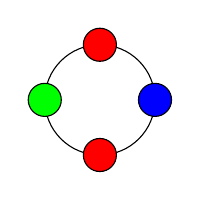
\begin{tikzpicture}[scale=0.7]
\draw[fill=white] (0,0) circle (1);
\draw[fill=red] (0,1) circle (0.3);
\draw[fill=blue] (1,0) circle (0.3);
\draw[fill=red] (0,-1) circle (0.3);
\draw[fill=green] (-1,0) circle (0.3);
\end{tikzpicture}
\end{center}
ima sljedeće simetrične ogrlice:
\begin{center}
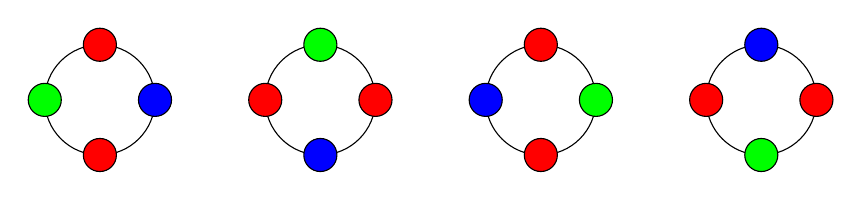
\begin{tikzpicture}[scale=0.7]
\draw[fill=white] (0,0) circle (1);
\draw[fill=red] (0,1) circle (0.3);
\draw[fill=blue] (1,0) circle (0.3);
\draw[fill=red] (0,-1) circle (0.3);
\draw[fill=green] (-1,0) circle (0.3);

\draw[fill=white] (4,0) circle (1);
\draw[fill=green] (4+0,1) circle (0.3);
\draw[fill=red] (4+1,0) circle (0.3);
\draw[fill=blue] (4+0,-1) circle (0.3);
\draw[fill=red] (4+-1,0) circle (0.3);

\draw[fill=white] (8,0) circle (1);
\draw[fill=red] (8+0,1) circle (0.3);
\draw[fill=green] (8+1,0) circle (0.3);
\draw[fill=red] (8+0,-1) circle (0.3);
\draw[fill=blue] (8+-1,0) circle (0.3);

\draw[fill=white] (12,0) circle (1);
\draw[fill=blue] (12+0,1) circle (0.3);
\draw[fill=red] (12+1,0) circle (0.3);
\draw[fill=green] (12+0,-1) circle (0.3);
\draw[fill=red] (12+-1,0) circle (0.3);
\end{tikzpicture}
\end{center}
Postoji $n$ načina promjene pozicije
ogrlice,
jer je možemo rotirati
$0,1,\ldots,n-1$ koraka u smjeru kazaljke na satu.
Ako je broj koraka 0,
svih $m^n$ ogrlica ostaje istima,
a ako je broj koraka 1,
samo $m$ ogrlica u kojima svaka
perla ima istu boju ostaje istima.

Općenitije, kada je broj koraka $k$,
ukupno
\[m^{\textrm{gcd}(k,n)}\]
ogrlica ostaje istima,
gdje je $\textrm{gcd}(k,n)$ najveći zajednički
djelitelj brojeva $k$ i $n$.
Razlog tome je da će blokovi
perli veličine $\textrm{gcd}(k,n)$
zamijeniti jedni druge.
Stoga je, prema Burnsideovoj lemi,
broj ogrlica
\[\sum_{i=0}^{n-1} \frac{m^{\textrm{gcd}(i,n)}}{n}. \]
Na primjer, broj ogrlica duljine 4
s 3 boje je
\[\frac{3^4+3+3^2+3}{4} = 24. \]

\section{Cayleyjeva formula}

\index{Cayleyjeva formula}

\key{Cayleyjeva formula}
% \footnote{While the formula is named after A. Cayley,
% who studied it in 1889, it was discovered earlier by C. W. Borchardt in 1860.}
kaže da
postoji $n^{n-2}$ označenih stabala
koja sadrže $n$ čvorova.
Čvorovi su označeni brojevima $1,2,\ldots,n$,
a dva stabla su različita
ako se razlikuju po strukturi ili
po označavanju.

\begin{samepage}
Na primjer, kada je $n=4$, broj označenih
stabala je $4^{4-2}=16$:

\begin{center}
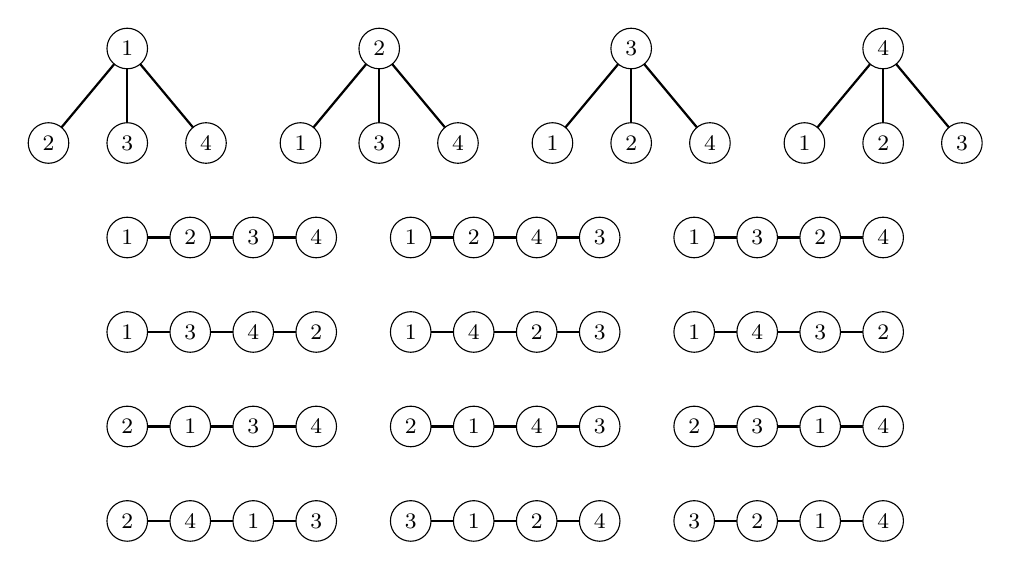
\begin{tikzpicture}[scale=0.8]
\footnotesize

\newcommand\puua[6]{
\path[draw,thick,-] (#1,#2) -- (#1-1.25,#2-1.5);
\path[draw,thick,-] (#1,#2) -- (#1,#2-1.5);
\path[draw,thick,-] (#1,#2) -- (#1+1.25,#2-1.5);
\node[draw, circle, fill=white] at (#1,#2) {#3};
\node[draw, circle, fill=white] at (#1-1.25,#2-1.5) {#4};
\node[draw, circle, fill=white] at (#1,#2-1.5) {#5};
\node[draw, circle, fill=white] at (#1+1.25,#2-1.5) {#6};
}
\newcommand\puub[6]{
\path[draw,thick,-] (#1,#2) -- (#1+1,#2);
\path[draw,thick,-] (#1+1,#2) -- (#1+2,#2);
\path[draw,thick,-] (#1+2,#2) -- (#1+3,#2);
\node[draw, circle, fill=white] at (#1,#2) {#3};
\node[draw, circle, fill=white] at (#1+1,#2) {#4};
\node[draw, circle, fill=white] at (#1+2,#2) {#5};
\node[draw, circle, fill=white] at (#1+3,#2) {#6};
}

\puua{0}{0}{1}{2}{3}{4}
\puua{4}{0}{2}{1}{3}{4}
\puua{8}{0}{3}{1}{2}{4}
\puua{12}{0}{4}{1}{2}{3}

\puub{0}{-3}{1}{2}{3}{4}
\puub{4.5}{-3}{1}{2}{4}{3}
\puub{9}{-3}{1}{3}{2}{4}
\puub{0}{-4.5}{1}{3}{4}{2}
\puub{4.5}{-4.5}{1}{4}{2}{3}
\puub{9}{-4.5}{1}{4}{3}{2}
\puub{0}{-6}{2}{1}{3}{4}
\puub{4.5}{-6}{2}{1}{4}{3}
\puub{9}{-6}{2}{3}{1}{4}
\puub{0}{-7.5}{2}{4}{1}{3}
\puub{4.5}{-7.5}{3}{1}{2}{4}
\puub{9}{-7.5}{3}{2}{1}{4}
\end{tikzpicture}
\end{center}
\end{samepage}

Zatim ćemo vidjeti kako se Cayleyjeva formula može
izvesti pomoću Prüferovih kodova.

\subsubsection{Prüferov kod}

\index{Prüferov kod}

\key{Prüferov kod}
%\footnote{In 1918, H. Prüfer proved Cayley's theorem using Prüfer codes \cite{pru18}.}
je slijed od
$n-2$ brojeva koji opisuje označeno stablo.
Kod se konstruira postupkom
koji uklanja $n-2$ listova iz stabla.
U svakom koraku uklanja se list s najmanjom oznakom,
a oznaka njegovog jedinog susjeda dodaje se u kod.

Na primjer, izračunajmo Prüferov kod
sljedećeg grafa:
\begin{center}
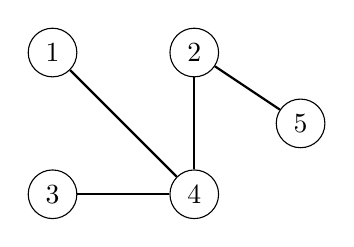
\begin{tikzpicture}[scale=0.9]
\node[draw, circle] (1) at (2,3) {$1$};
\node[draw, circle] (2) at (4,3) {$2$};
\node[draw, circle] (3) at (2,1) {$3$};
\node[draw, circle] (4) at (4,1) {$4$};
\node[draw, circle] (5) at (5.5,2) {$5$};

\path[draw,thick,-] (1) -- (4);
\path[draw,thick,-] (3) -- (4);
\path[draw,thick,-] (2) -- (4);
\path[draw,thick,-] (2) -- (5);
\end{tikzpicture}
\end{center}

Prvo uklanjamo čvor 1 i dodajemo čvor 4 u kod:
\begin{center}
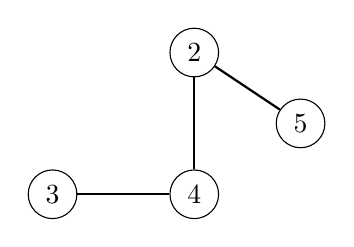
\begin{tikzpicture}[scale=0.9]
%\node[draw, circle] (1) at (2,3) {$1$};
\node[draw, circle] (2) at (4,3) {$2$};
\node[draw, circle] (3) at (2,1) {$3$};
\node[draw, circle] (4) at (4,1) {$4$};
\node[draw, circle] (5) at (5.5,2) {$5$};

%\path[draw,thick,-] (1) -- (4);
\path[draw,thick,-] (3) -- (4);
\path[draw,thick,-] (2) -- (4);
\path[draw,thick,-] (2) -- (5);
\end{tikzpicture}
\end{center}

Zatim uklanjamo čvor 3 i dodajemo čvor 4 u kod:
\begin{center}
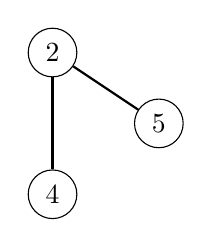
\begin{tikzpicture}[scale=0.9]
%\node[draw, circle] (1) at (2,3) {$1$};
\node[draw, circle] (2) at (4,3) {$2$};
%\node[draw, circle] (3) at (2,1) {$3$};
\node[draw, circle] (4) at (4,1) {$4$};
\node[draw, circle] (5) at (5.5,2) {$5$};

%\path[draw,thick,-] (1) -- (4);
%\path[draw,thick,-] (3) -- (4);
\path[draw,thick,-] (2) -- (4);
\path[draw,thick,-] (2) -- (5);
\end{tikzpicture}
\end{center}

Na kraju uklanjamo čvor 4 i dodajemo čvor 2 u kod:
\begin{center}
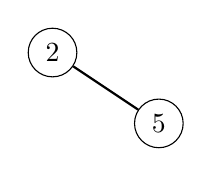
\begin{tikzpicture}[scale=0.9]
%\node[draw, circle] (1) at (2,3) {$1$};
\node[draw, circle] (2) at (4,3) {$2$};
%\node[draw, circle] (3) at (2,1) {$3$};
%\node[draw, circle] (4) at (4,1) {$4$};
\node[draw, circle] (5) at (5.5,2) {$5$};

%\path[draw,thick,-] (1) -- (4);
%\path[draw,thick,-] (3) -- (4);
%\path[draw,thick,-] (2) -- (4);
\path[draw,thick,-] (2) -- (5);
\end{tikzpicture}
\end{center}

Stoga je Prüferov kod grafa $[4,4,2]$.

Prüferov kod možemo konstruirati za bilo koje stablo,
i još važnije,
izvorno stablo može se rekonstruirati
iz Prüferovog koda.
Dakle, broj označenih stabala
s $n$ čvorova jednak je
$n^{n-2}$, broju Prüferovih kodova
veličine $n$.
